\documentclass[12pt]{article}
\usepackage[utf8]{inputenc}
\usepackage[spanish]{babel}
\decimalpoint
\usepackage{mathtools}
\usepackage{amsmath}
\usepackage{amsthm}
\usepackage{amssymb}
\usepackage{graphicx}
\usepackage[margin=0.9in]{geometry}
\usepackage{fancyhdr}
\usepackage[inline]{enumitem}
\usepackage{float}
\usepackage{cancel}
\usepackage{bigints}
\usepackage{color}
\usepackage{xcolor}
\usepackage{listingsutf8}
\usepackage{algorithm}
\usepackage{tocloft}
\usepackage[none]{hyphenat}
\usepackage{graphicx}
\usepackage{grffile}
\usepackage{tabularx}
\usepackage[nottoc,notlot,notlof]{tocbibind}
\usepackage{times}
\usepackage{color}
\definecolor{gray97}{gray}{.97}
\definecolor{gray75}{gray}{.75}
\definecolor{gray45}{gray}{.45}
\renewcommand{\cftsecleader}{\cftdotfill{\cftdotsep}}
\pagestyle{fancy}
\setlength{\headheight}{15pt} 
\lhead{Operaciones con cadenas}
\rhead{\thepage}
\lfoot{ESCOM-IPN}
\renewcommand{\footrulewidth}{0.5pt}
\setlength{\parskip}{0.5em}
\newcommand{\ve}[1]{\overrightarrow{#1}}
\newcommand{\abs}[1]{\left\lvert #1 \right\lvert}
\date{ 8 de Marzo 2018}
\title{Expresión Regular}
\author{Reporte 2}

\definecolor{pblue}{rgb}{0.13,0.13,1}
\definecolor{pgreen}{rgb}{0,0.5,0}
\definecolor{pred}{rgb}{0.9,0,0}
\definecolor{pgrey}{rgb}{0.46,0.45,0.48}
\lstset{tabsize=1}

\usepackage{listings}
\lstset{ frame=Ltb,
framerule=0pt,
aboveskip=0.5cm,
framextopmargin=3pt,
framexbottommargin=3pt,
framexleftmargin=0.4cm,
framesep=0pt,
rulesep=.4pt,
backgroundcolor=\color{gray97},
rulesepcolor=\color{black},
%
stringstyle=\ttfamily,
showstringspaces = false,
basicstyle=\small\ttfamily,
commentstyle=\color{gray45},
keywordstyle=\bfseries,
%
numbers=left,
numbersep=15pt,
numberstyle=\tiny,
numberfirstline = false,
breaklines=true,
}

% minimizar fragmentado de listados
\lstnewenvironment{listing}[1][]
{\lstset{#1}\pagebreak[0]}{\pagebreak[0]}

\lstdefinestyle{consola}
{basicstyle=\scriptsize\bf\ttfamily,
backgroundcolor=\color{gray75},
}

\lstdefinestyle{Java}
{language=Java,
}

%%%%%%%%%%%%%%%%%%%%%

\lstdefinestyle{customc}{
  belowcaptionskip=1\baselineskip,
  breaklines=true,
  frame=L,
  xleftmargin=\parindent,
  language=C,
  showstringspaces=false,
  basicstyle=\footnotesize\ttfamily,
  keywordstyle=\bfseries\color{green!40!black},
  commentstyle=\itshape\color{purple!40!black},
  identifierstyle=\color{blue},
  stringstyle=\color{orange},
}

\lstdefinestyle{customasm}{
  belowcaptionskip=1\baselineskip,
  frame=L,
  xleftmargin=\parindent,
  language=[x86masm]Assembler,
  basicstyle=\footnotesize\ttfamily,
  commentstyle=\itshape\color{purple!40!black},
}

\lstset{escapechar=@,style=customc}

%Permite crear columnas en el documento
\usepackage{multicol} 
\usepackage{color}
\usepackage{comment}
\newcommand{\tabitem}{~~\llap{\textbullet}~~}
\newcommand{\subtabitem}{~~~~\llap{\textbullet}~~}

\bibliographystyle{IEEEtran}
\begin{document}
		\begin{titlepage}
			\begin{center}
				
				% Upper part of the page. The '~' is needed because \\
				% only works if a paragraph has started.
				
				\noindent
				\begin{minipage}{0.5\textwidth}
					\begin{flushleft} \large
						\includegraphics[width=0.3\textwidth]{../ipn.png}
					\end{flushleft}
				\end{minipage}%
				\begin{minipage}{0.55\textwidth}
					\begin{flushright} \large
						\includegraphics[width=0.7\textwidth]{../escom.png}
					\end{flushright}
				\end{minipage}
				
				\textsc{\LARGE Instituto Politécnico Nacional}\\[0.5cm]
				
				\textsc{\Large Escuela Superior de Cómputo}\\[1cm]
				
				% Title
				
				{ \huge Práctica 2 - Expresión Regular \\[1cm] }
				
				{ \Large Unidad de aprendizaje: Teoría computacional} \\[1cm]
				
				{ \Large Grupo: 2CM4 } \\[1cm]
				
				\noindent
				\begin{minipage}{0.5\textwidth}
					\begin{flushleft} \large
						\emph{Alumno(a):}\\
						
						\begin{tabular}{ll}
					     Nicolás Sayago Abigail\\
					\end{tabular}
					\end{flushleft}
				\end{minipage}%
				\begin{minipage}{0.5\textwidth}
					\begin{flushright} \large
						\emph{Profesor(a):} \\
						Sanchez García Luz María  \\
					\end{flushright}
				\end{minipage}
				
				\vfill
				
				% Bottom of the page
				{\large 8 de Marzo de 2018}
			\end{center}
		\end{titlepage}
	
	\tableofcontents
	\newpage
	% \\\\\\\\\\\\\\\\\\\\\\\\\\\\\\\\\\\\\\\\\\\\\\\\\\\\\\\\\\\\
	% \\\\\\\\\\\\\\\\\\\\\\\ INTRODUCCION \\\\\\\\\\\\\\\\\\\\\\\
	% \\\\\\\\\\\\\\\\\\\\\\\\\\\\\\\\\\\\\\\\\\\\\\\\\\\\\\\\\\\\

	\section{Introducción}
	En la siguiente práctica se implementara una expresión regular en el lenguaje de programación de JAVA.
	La expresión regular sera de un número de boleta que pertenece a un Sistema Administrativo y Escolar 
	de Educación Básica (SAEEB), que está siendo desarrollado.

	A lo largo del documento usaremos la palabra \textbf{Expresión Regular}, por lo cual tenemos que definir
	¿Qué es una expresión regular?.

	\subsection{Expresión regular}
	
	Una \textbf{expresión regular} es una forma abreviada de representar cadenas de caracteres que se ajustan
	a un determinado patrón. Al conjunto de cadenas representado por la expresión \textsl{r} se lo llama 
	\textsl{lenguaje generado por la expresión regular r}  y se escribe \textsl{L(r)}. Una expresión regular 
	se define sobre un alfabeto \ y es una cadena formada por caracteres de dicho alfabeto y por una serie de
	operadores también llamadas metacaracteres.
	Una expresión regular define un patrón de búsqueda para cadenas de caracteres. Los podemos utilizar 	
	para comprobar si una cadena contiene o coincide con el patrón. El
	contenido de caracteres puede
	coincidir con el patron 0, 1 o más veces.

	\subsection{Expresión regular en programación}

	Los usos de las expresiones regulares son muchos, por ejemplo, en algunos lenguajes de programación
	las expresiones regulares sirven para detectar patrones en distintas cadenas de texto. Para los
	programadores, esas expresiones regulares facilitan su labor en un solo paso. Un ejemplo muy sencillo
	es la comprobación vía expresión regular que los datos rellenados por los usuarios en un formulario 
	son correctos o no. Alguien puede utilizar un breve formulario para recabar el nombre, los apellidos 
	y el teléfono de contacto de sus clientes, y que algunos de ellos no completen bien este ultimo campo.
	La forma rápida de comprobarlo es a través de una expresión regular.

	Algunos otros ejemplos de uso de expresiones regulares pueden ser:

	\begin{itemize}
		\item[$\rightarrow$] Comprobar que la fecha leída cumple el patrón dd/mm/aaaa
		\item[$\rightarrow$] Comprobar que un NIF esta formado por 8 cifras, un guión y una letra
		\item[$\rightarrow$] Comprobar que una dirección de correo es válida
		\item[$\rightarrow$] Comprobar que una contraseña cumple unas determinadas condiciones.
		\item[$\rightarrow$] Comprobar que una URL es válida.
	\end{itemize} 

	\newpage
	% \\\\\\\\\\\\\\\\\\\\\\\\\\\\\\\\\\\\\\\\\\\\\\\\\\\\\\\\\\\\\\\\\\\\\\\\\\
	% \\\\\\\\\\\\\\\\\\\\\\\ PLANTEAMIENTO DEL PROBLEMA \\\\\\\\\\\\\\\\\\\\\\\
	% \\\\\\\\\\\\\\\\\\\\\\\\\\\\\\\\\\\\\\\\\\\\\\\\\\\\\\\\\\\\\\\\\\\\\\\\\\

	\section{Planteamiento del problema}
	De forma general la expresión regular elegida define un número de identificación para un alumno que 
	pertence a una escuela secundaria publica, debido a esto su numero de boleta estará dado por:
	\begin{itemize}
		\item Año de ingreso.										
		\item Número de entidad federativa. 						
		\item Número de municipio en esa entidad federativa.		
		\item Número de escuela en ese municipio.					
		\item Puede ser Alumno o Docente, siendo identificados con A y D respectivamente.	
		\item Número de usuario dado por 3 números y una letra.								
	\end{itemize}
	Para esta práctica delimitamos el número de boleta para un alumno del Estado de México.
	Así que diseñamos la solución para implementar la expresión regular definida por lo siguiente:

	\begin{itemize}
		\item Niños que hayan ingresado en los años 2014-2017.								
		\item Que la escuela pertenezca a la entidad federativa Estado de México. 			
		\item Que sea de uno de los 125 municipios de esa entidad federativa.				
		\item Pertenezca a una de las escuelas en ese municipio (0-99)						
		\item Puede ser Alumno o Docente, siendo identificados con A y D respectivamente.	
		\item Número de usuario dado por 3 números y una letra.	(Identificador).							
		\item Tiene un total de 16 caracteres.
	\end{itemize}

	\begin{figure}[H]
	        \centering
	        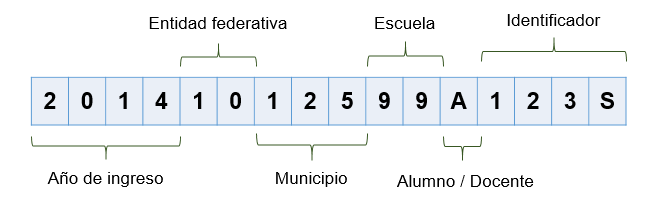
\includegraphics[scale=0.9]{Practica2/Estructura.PNG}
	\end{figure}
    \newpage
	\begin{multicols}{2}[Algunos ejemplos son:]
		Cadenas validas son:
		\begin{itemize}
			\item 20141012599A123A
			\item 20141012599D144A
			\item 20151000198A126R
			\item 20171003474A112D
		\end{itemize}
		\columnbreak
		Cadenas no validas:
		\begin{itemize}
			\item 20181312599S123A12  
			\item 20171013515D014S    
			\item 20141012599A13S$<$  
			\item 20131012610D123A  
			\end{itemize}
	\end{multicols}
	\newpage
	A continuación se ve la tabla que permite determinar el número de estado que tendrá asignado,
	así como también el número de municipios que se permite por entidad Federativa. Observamos
	unicamente la del Estado de México, aunque también cabe señalar que si se quiere implementar
	una expresión regular con cualquier otro estado, se podría de manera similar a la que vamos a 
	hacer. 

	\begin{table}[H]
        \begin{tabular}{|p{4cm}|p{8cm}|p{4cm}|}
        \hline
            \textbf{No.}	& \textbf{Entidad Federativa}& 	\textbf{Municipio} \\ \hline
            	1 			&	Aguascalientes 			&			1			\\ \hline
                2			&	Baja California 		& 			5 			\\ \hline
            	3			&	Baja California Sur  	&			5 			\\ \hline
            	4			&	Campeche				&			11 			\\ \hline
            	5			&	Chiapas					&			122			\\ \hline
            	6			&	Chihuahua				&			67			\\ \hline
            	7			&	Coahuila 				&			38			\\ \hline
            	8			&	Colima					&			10			\\ \hline
            	9			&	Durango					&			39			\\ \hline
            	10			&	Estado de México		&			125			\\ \hline
            	11			&	Guanajuato				&			46			\\ \hline
            	12			&	Guerrero				&			81			\\ \hline
            	13			&	Hidalgo					&			84			\\ \hline
            	14			&	Jalisco					&			125			\\ \hline
            	15			&	Michoacán				&			113			\\ \hline
            	16			&	Morelos					&			33			\\ \hline
            	17			&	Nayarit					&			20			\\ \hline
            	18			&	Nuevo León				&			51			\\ \hline
            	19			&	Oaxaca					&			570			\\ \hline
            	20			&	Puebla					&			217			\\ \hline
            	21			&	Querétaro				&			18			\\ \hline
            	22			&	Quintana Roo			&			11			\\ \hline
            	23			&	San Luis Potosí			&			58			\\ \hline
            	24			&	Sinaloa					&			18			\\ \hline
            	25			&	Sonora					&			72			\\ \hline
            	26			&	Tabasco					&			17			\\ \hline
            	27			&	Tamaulipas				&			43			\\ \hline
            	28			&	Tlaxcala				&			60			\\ \hline
            	29			&	Veracruz				&			212			\\ \hline
            	30			&	Yucatán					&			106			\\ \hline
            	31			&	Zacatecas				&			58			\\ \hline
            	32			&	Ciudad de México		&			16			\\ \hline
        \end{tabular}
    \end{table}
	\newpage
	% \\\\\\\\\\\\\\\\\\\\\\\\\\\\\\\\\\\\\\\\\\\\\\\\\\\\\\\\\\\\\\\\\\\\\
	% \\\\\\\\\\\\\\\\\\\\\\\ DISEÑO DE LA SOLUCION \\\\\\\\\\\\\\\\\\\\\\\
	% \\\\\\\\\\\\\\\\\\\\\\\\\\\\\\\\\\\\\\\\\\\\\\\\\\\\\\\\\\\\\\\\\\\\\\

	\section{Diseño de la solución}

	A continuación mostraré el diseño que se tiene para implementar la solución, dados
	los requerimientos expresados antes.
	La expresión regular es:

	\begin{equation*}
		20\left[ 4-7\rigth] 10([0-1][0-9][0-9])([0-9][1-9])[AD][0-9][0-9][0-9][A-Z]
	\end{equation*}

	% \\\\\\\\\\\\\\\\\\\\\\\\\\\\\\\\\\\\\\\\\\\\\\\\\\\\\\\\\\\\\\\\\\\\\\\\\\\\\
	% \\\\\\\\\\\\\\\\\\\\\\\ IMPLEMENTACION DE LA SOLUCION \\\\\\\\\\\\\\\\\\\\\\\
	% \\\\\\\\\\\\\\\\\\\\\\\\\\\\\\\\\\\\\\\\\\\\\\\\\\\\\\\\\\\\\\\\\\\\\\\\\\\\\

	\section{Implementación de la solución}

	Primero muestro una tabla con los métodos con los que ya cuenta el 
	lenguaje de programación y que fueron utilizados en la realización 
	de la implementación de la práctica.

	 \begin{table}[H]
        \begin{tabular}{|p{6.5cm}|p{9.5cm}|}
        \hline
            \textbf{Método} & \textbf{Función} \\ \hline
            Pattern			& El método pattern devuelve la expresión regular que hemos compilado. \\ \hline
            Pattern.matcher & Nos permite realizar operaciones sobre la secuencia de caracteres que queremos validar o la secuencia de caracteres en la que queremos buscar. \\ \hline
            cadena.charAr(indice) & Devuelve el caracter que encuentra en una posición especifica. \\ \hline
        \end{tabular}
    \end{table}

	De forma general el programa esta estructurado de tal forma que al dar click al boton \textbf{OK} haga algunas validaciones como son la longitud y el número de municipio, si pasa ese filtro, entonces manda al método \textbf{ValidarExpresion} la cadena a validar totalmente.

	El método \textbf{ValidarExpresion} contiene una cadena que es prácticamente la expresión regular del número de alumno después se usa el método \textbf{Pattern.compile}  que \textsl{compila} nuestra expresión regular. Posteriormente con el método \textbf{Matcher} se comprueban las cadenas contra el patrón indicado.

	Cabe señalar que con el método \textbf{ValidarExpresion} era más que suficiente, sin embargo podemos evitar que se haga todo un desgaste de memoria haciendo ciertos \textbf{\textsl{filtros}} al recibir la cadena como la de la longitud

	\newpage
	\begin{itemize}
		\item IMPLEMENTACIÓN AL HACER CLIK AL BOTÓN
		\begin{lstlisting}[style=Java]
	public void actionPerformed(ActionEvent e)
	{
		JButton b = (JButton)e.getSource(); // Recibimos un boton
		String aux="";
		Boolean a; // Bandera
		int aux2, i;
		if(b == Enviar) // Si el boton es el de enviar
		{	
			a = true;
			// Obtenemos la cadena a validar
			String cad = Cadena.getText(); 
			// Si la cadena es de longitud 16 
			if(cad.length() == 16)
			{	
				// Obtenemos el número de municipio
				for(i=6; i<9; i++) 
					aux = aux + cad.charAt(i);
				aux2 = Integer.parseInt(aux);
				if (aux2 < 126) // Si el número de municipio esta en el rango
				{
					// Finalmente mandamos la cadena 
					if(a = validarExpresion(cad)) 
						Valida.setText("CADENA VALIDA");
					else // Si no cumple con la E.R
						Valida.setText("CADENA NO VALIDA");	
				}
				else // Si el municipio no esta en el rango
					Valida.setText("CADENA NO VALIDA");
			} 
			else // Si la cadena no es de longitud 16
				Valida.setText("CADENA NO VALIDA");
		}
	}
		\end{lstlisting}			

		\item IMPLEMENTACIÓN DEL MÉTODO VALIDAR EXPRESIÓN
	
	\begin{lstlisting}[style=Java]
	private boolean validarExpresion(String CAD)
	{   // Generamos la expresión regular
		String regex = "([2]{1}[0]{1})(1[4-7])" + 
						"1" + "0" + 
						"([0-1][0-9][0-9])" + 
						"([0-9][1-9])" + 
						"[AD]{1}" + 
						"[0-9][0-9][0-9][A-Z]{1}" ;
		// Se compila la expresión regular
		Pattern patron = Pattern.compile(regex);
		// Si la cadena no coincide con la expresión regular
		if(!patron.matcher(CAD).matches()) 
			return false;
		else
			return true;
	}
	\end{lstlisting}

	\end{itemize}
		

	% \\\\\\\\\\\\\\\\\\\\\\\\\\\\\\\\\\\\\\\\\\\\\\\\\\\\\\\\\\\\\\
	% \\\\\\\\\\\\\\\\\\\\\\\ FUNCIONAMIENTO \\\\\\\\\\\\\\\\\\\\\\\
	% \\\\\\\\\\\\\\\\\\\\\\\\\\\\\\\\\\\\\\\\\\\\\\\\\\\\\\\\\\\\\\

	\section{Funcionamiento}
	Primero que nada, mostramos la interfaz inicial. Observamos que el 
	usuario tiene la oportunidad de ingresar una cadena. Al dar click en el botón OK, se mostrará
	\textbf{CADENA VALIDA} si la cadena que se ha ingresado cumple con el formato del número de boleta
	en caso contrario, se mostrará \textbf{CADENA NO VALIDA}.

	La pantalla inicial es la siguiente:
	
	\begin{figure}[H]
	        \centering
	        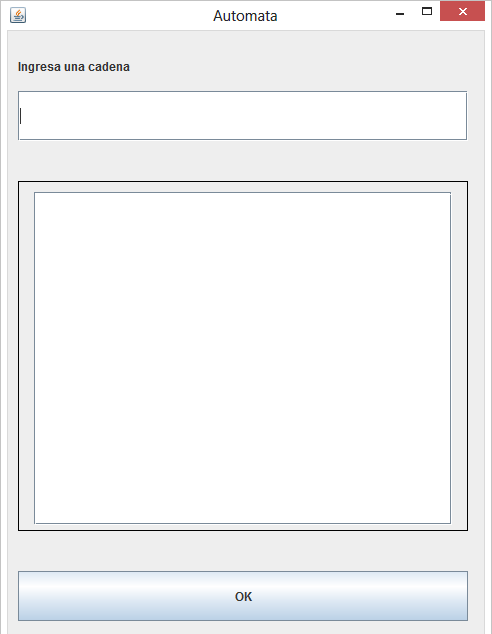
\includegraphics[scale=0.9]{Practica2/F_1.PNG}
	\end{figure}
	
	A continuación muestro ejemplos de \textbf{cadenas validas}:
	\begin{figure}[H]
	        \centering
	        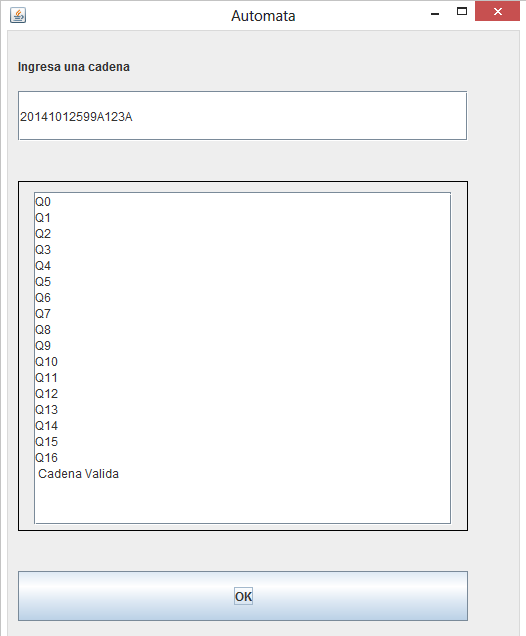
\includegraphics[scale=0.9]{Practica2/F_2.PNG}
	\end{figure}
	
	\begin{figure}[H]
	        \centering
	        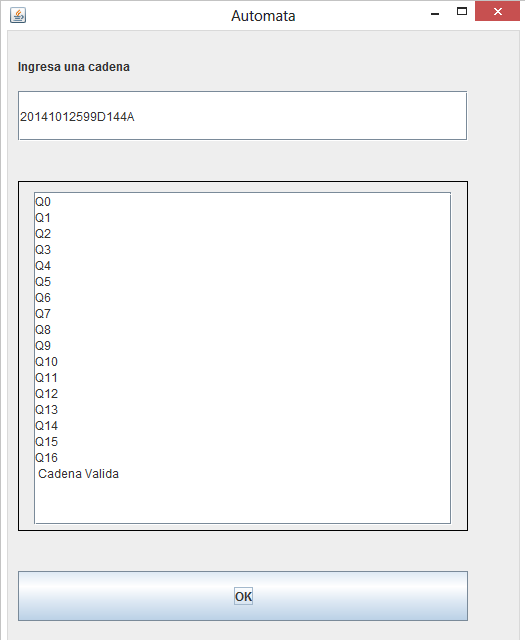
\includegraphics[scale=0.9]{Practica2/F_3.PNG}
	\end{figure}

	\begin{figure}[H]
	        \centering
	        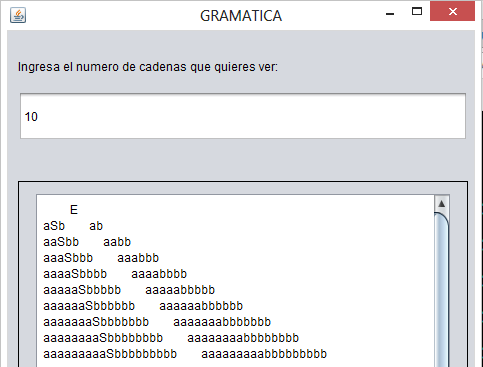
\includegraphics[scale=0.9]{Practica2/F_4.PNG}
	\end{figure}

	\begin{figure}[H]
	        \centering
	        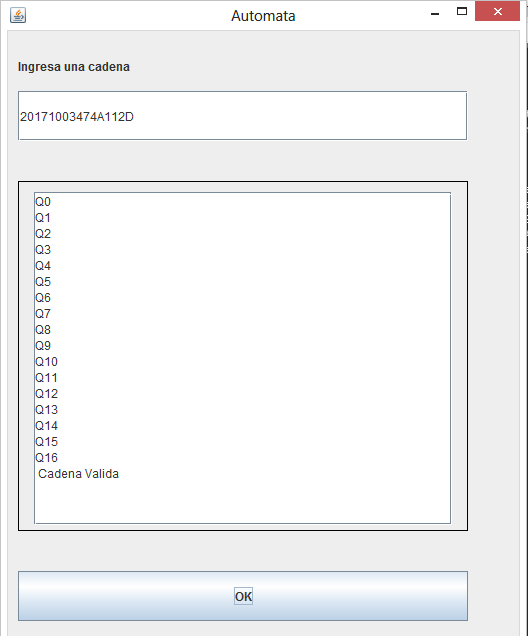
\includegraphics[scale=0.9]{Practica2/F_5.PNG}
	\end{figure}

	Ahora ejemplos de \textbf{cadenas no validas}:
	\begin{figure}[H]
	        \centering
	        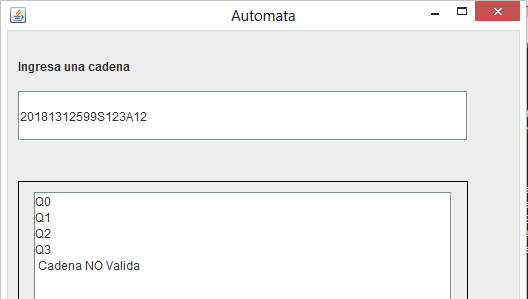
\includegraphics[scale=0.9]{Practica2/F_6.PNG}
	\end{figure}

	\begin{figure}[H]
	        \centering
	        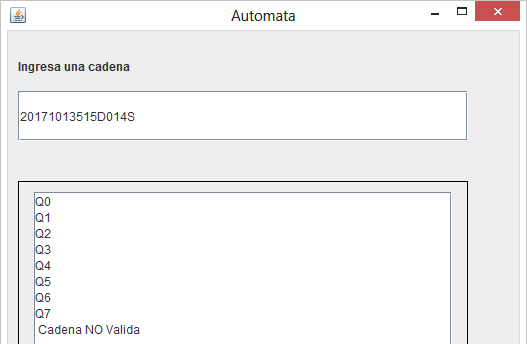
\includegraphics[scale=0.9]{Practica2/F_7.PNG}
	\end{figure}

	\begin{figure}[H]
	        \centering
	        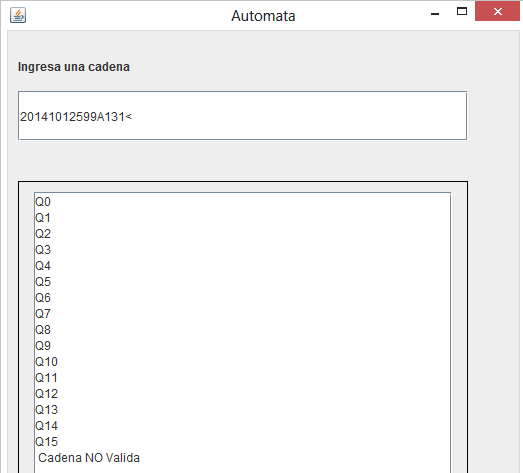
\includegraphics[scale=0.9]{Practica2/F_8.PNG}
	\end{figure}

	\begin{figure}[H]
	        \centering
	        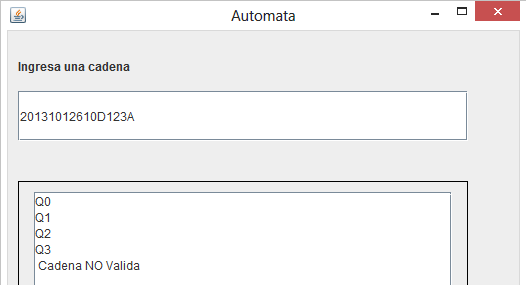
\includegraphics[scale=0.9]{Practica2/F_9.PNG}
	\end{figure}

	% \\\\\\\\\\\\\\\\\\\\\\\\\\\\\\\\\\\\\\\\\\\\\\\\\\\\\\\\\\\\
	% \\\\\\\\\\\\\\\\\\\\\\\ CONCLUSIONES \\\\\\\\\\\\\\\\\\\\\\\
	% \\\\\\\\\\\\\\\\\\\\\\\\\\\\\\\\\\\\\\\\\\\\\\\\\\\\\\\\\\\\

	\section{Conclusiones}

	Al terminar está práctica pude observar la importancia de las expresiones regulares y la forma en la que 
	son ocupadas para validar cadenas, especialmente porque las condiciones las especifique yo puesto que 
	dichos número sde boleta serán ocupados en un sistema que será implementado en la clase de Análisis
	de Diseño Orientado a Objetos, así que usare lo desarrollado en está práctica para el sistema y las 
	validaciones. 


	% \\\\\\\\\\\\\\\\\\\\\\\\\\\\\\\\\\\\\\\\\\\\\\\\\\\\\\\\\\\\
	% \\\\\\\\\\\\\\\\\\\\\\\ BIBLIOGRAFIA \\\\\\\\\\\\\\\\\\\\\\\
	% \\\\\\\\\\\\\\\\\\\\\\\\\\\\\\\\\\\\\\\\\\\\\\\\\\\\\\\\\\\\

	 \nocite{ref1, ref2}
	\bibliography{referencias}
\end{document}